\section{Problem Description}

A subway system is composed of trains, passengers, tracks and stations. The
purpose of the subway system is to transport passengers from one station to
their desired station. Tracks connect stations and trains travel station to
station. Trains may only overtake one another if the track section or station
they are both on has a passing area. Trains have a passenger capacity. When a
train arrives at a station it has a fixed amount of time for passengers to
embark and disembark. It is assumed that everyone that wants to disembark gets
an opportunity to do so before people are given an opportunity to embark. Since
embarking and disembarking of passengers from a train takes time and the train
has a fixed capacity not everyone that wants to embark or disembark may be get
an opportunity to do so. Trains have a possibility to be delayed or broken down.
Delayed trains take longer to reach their destination. Broken down trains force
all passengers off the train when the train arrives at the nearest station and
then delays the train until it is repaired. Passengers are assumed to enter
stations at a fixed rate.

\subsection{Rail System Models}

A natural data structure choice for representing a rail system is a directed
graph.  In the most basic implementation, each station would be a vertex and the
edges would each represent a directional track from one station to the next.
Figure~\ref{fig:directedgraph} shows a directed graph model of the Sheppard Line
in the Toronto subway system.

\begin{figure}[htb]
	\centering
	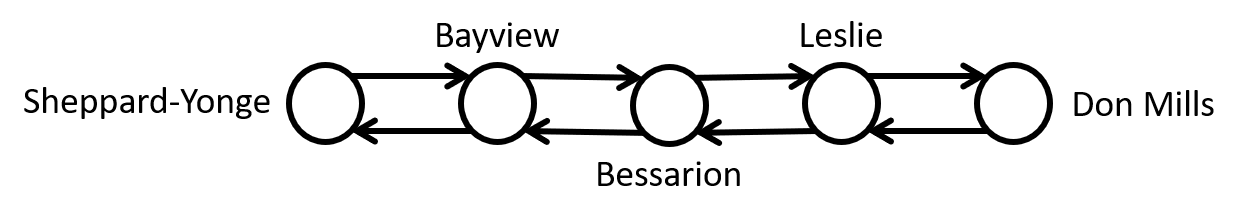
\includegraphics[width=6.5in]{directedgraph.png}
	\caption{Directed Graph Model of Sheppard Subway Line}
	\label{fig:directedgraph}
\end{figure}

What the directed graph representation lacks for this application is any notion
of an integrated train model. A separate train model could be made to use the
directed graph simply to know where to go next, but it would require much extra
logic to determine \textit{if} it could go do the next station.  Where this
decision is made is also not obvious when using the directed graph.

Similar to directed graphs and used in discrete event modeling of concurrent
systems is a structure called a Petri net.~\cite{Petri62}  Synonymous to the
vertices in a directed graph, Petri nets contain \textit{places}.  Whereas
directed graphs use edges to connect those vertices, Petri nets use
\textit{arcs}. However, Petri nets do not simply connect one \textit{place} to
another.  \textit{Arcs} actually connect \textit{places} to
\textit{transitions}. Each \textit{transition} has an input and an output arc
joining it to \textit{places}.  Each \textit{place} optionally can contain a
finite number of \textit{tokens}.  \textit{Tokens} for this application
represent the trains.  More formally, they are objects that represent processes
in a given state, where the states are represented by the
\textit{places}.~\cite{Kristoffersen2003}  Figure~\ref{fig:petrinet} shows a
Petri net model of the Sheppard subway line. The rectangles at the midpoint of
the arcs represent the transitions and the black dots inside the represent the
tokens.

\begin{figure}[htb]
	\centering
	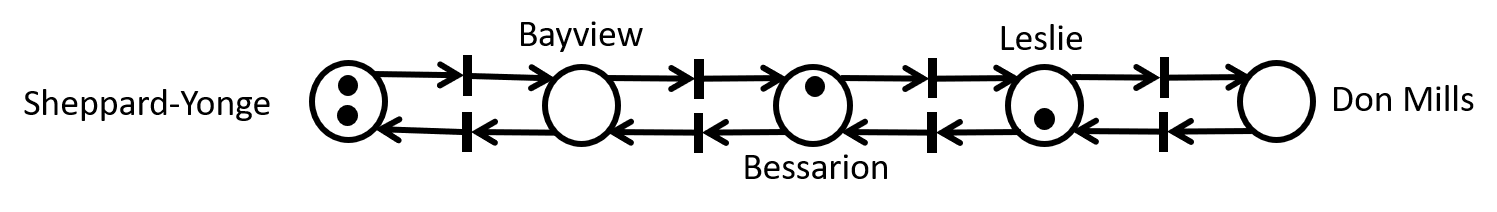
\includegraphics[width=6.5in]{petrinet.png}
	\caption{Petri Net Model of Sheppard Subway Line}
	\label{fig:directedgraph}
\end{figure}

\subsection{Train Movement Between Stations}

Train movement between stations must obey the physical layout of the track and
stations. Petri nets and collision detection are explored here as ways to
establish feasible and crash free subway dynamics.

Collision detection can ensure feasible, crash free subway dynamics by requiring
trains to be far enough apart that if one train stops the trains behind it do
not rear end it. Calculation of minimum distance between trains requires
information about track layout and train velocity and acceleration. A model of a
train traveling between stations has been done by Xu et al (2014). In their
model of a train between stations there is an acceleration period, a cruising
period and a deceleration period. Multiple trains traveling on the same track
can be modeled as a difference equation. At each step trains proceed to the next
station in a safe manner taking into account time and energy efficiency. The
safety criterion requires that the minimum stopping distance of the rear train
is less than the distance between the leader and follower train train plus the
minimum stopping distance of the lead train and a safety factor. 

Petri nets were chosen over collision detection for simulating subway train
movement because Petri nets are simpler, more efficient require less data to
calibrate and capture the dynamics of train break downs and delays. 

Petri nets are simpler than collision detection because Petri nets do not have
the detailed physics requirements of a collision detection model. In the
collision detection model minimum safe distance needs to be calculated by every
train at every time step. With a Petri net, minimum safe distance calculations
can be avoided by discretizing the track into sections with length greater than
the trains minimum stopping distance at maximum speed (or with a number of
sections if a more than one track lookahead rule is used) which ensures that
collisions are always avoidable. 

Petri nets are more efficient because they do not require any physics
calculations during simulation and can evaluated as discrete events which
results in a fewer number of calculations being required so long as track
sections are large relative to the size of the time steps in a collision model.

Petri nets are capable of modeling the break down and delay dynamics of interest
because a train delay or breakdown will back up the trains behind it so long as
the section of track the delayed or broken down train is on does not have a
passing track. 

More data is needed for a collision detection model because it has higher
physics fidelity than a Petri net. With the Petri net you only need the time it
takes to pass through a section of track and the minimum stopping distance at
maximum speed. The collision model requires knowledge of train accelaration and
deceleration and maximum speed at different locations on the track.
